\documentclass[a4paper,11pt]{article}
\input{/home/tof/Documents/Cozy/latex-include/preambule_lua.tex}
\newcommand{\showprof}{show them}  % comment this line if you don't want to see todo environment
\fancyhead[L]{Parcours}
\newdate{madate}{10}{09}{2020}
%\fancyhead[R]{\displaydate{madate}} %\today
%\fancyhead[R]{Seconde - SNT}
%\fancyhead[R]{Première - NSI}
\fancyhead[R]{Terminale - NSI}
\fancyfoot[L]{~\\Christophe Viroulaud}
\AtEndDocument{\label{lastpage}}
\fancyfoot[C]{\textbf{Page \thepage/\pageref{lastpage}}}
\fancyfoot[R]{\includegraphics[width=2cm,align=t]{/home/tof/Documents/Cozy/latex-include/cc.png}}
\usepackage{tikz}
\begin{document}
\begin{Form}
DFS à la main
\begin{center}
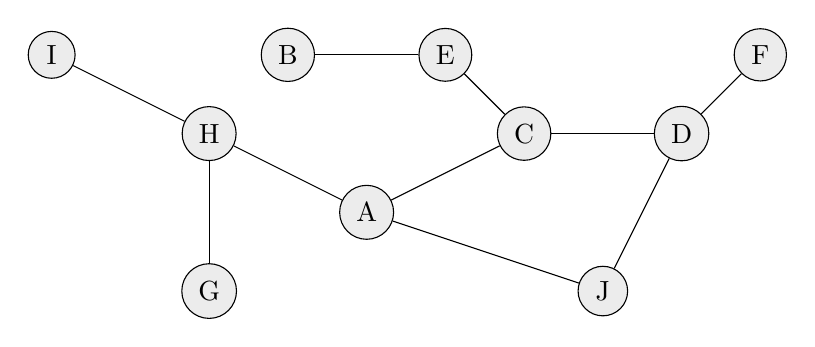
\begin{tikzpicture}
\node[draw,circle,fill=gray!15] (A)at(0,0) {A};
\node[draw,circle,fill=gray!15] (B)at(-1,2) {B};
\node[draw,circle,fill=gray!15] (C)at(2,1) {C};
\node[draw,circle,fill=gray!15] (D)at(4,1) {D};
\node[draw,circle,fill=gray!15] (E)at(1,2) {E};
\node[draw,circle,fill=gray!15] (F)at(5,2) {F};
\node[draw,circle,fill=gray!15] (G)at(-2,-1) {G};
\node[draw,circle,fill=gray!15] (H)at(-2,1) {H};
\node[draw,circle,fill=gray!15] (I)at(-4,2) {I};
\node[draw,circle,fill=gray!15] (J)at(3,-1) {J};
\draw[-,>=latex] (E) -- (B);
\draw[-,>=latex] (A) -- (C);
\draw[-,>=latex] (A) -- (H);
\draw[-,>=latex] (A) -- (J);
\draw[-,>=latex] (H) -- (I);
\draw[-,>=latex] (H) -- (G);
\draw[-,>=latex] (C) -- (E);
\draw[-,>=latex] (C) -- (D);
%\draw[-,>=latex] (C) -- (J);
\draw[-,>=latex] (D) -- (J);
\draw[-,>=latex] (D) -- (F);
\end{tikzpicture}
\end{center}
\begin{center}
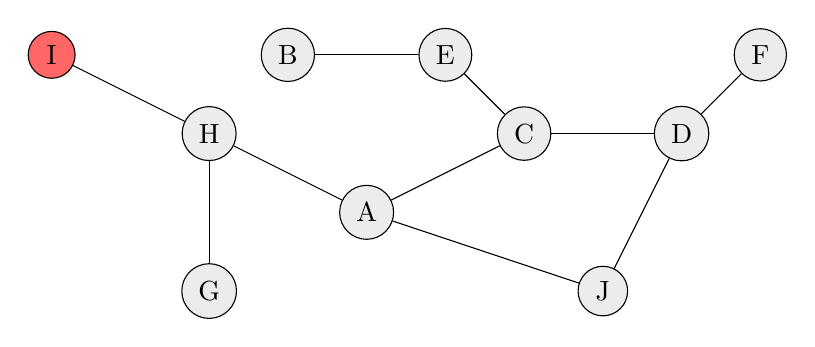
\begin{tikzpicture}
\node[draw,circle,fill=gray!15] (A)at(0,0) {A};
\node[draw,circle,fill=gray!15] (B)at(-1,2) {B};
\node[draw,circle,fill=gray!15] (C)at(2,1) {C};
\node[draw,circle,fill=gray!15] (D)at(4,1) {D};
\node[draw,circle,fill=gray!15] (E)at(1,2) {E};
\node[draw,circle,fill=gray!15] (F)at(5,2) {F};
\node[draw,circle,fill=gray!15] (G)at(-2,-1) {G};
\node[draw,circle,fill=gray!15] (H)at(-2,1) {H};
\node[draw,circle,fill=red!60] (I)at(-4,2) {I};
\node[draw,circle,fill=gray!15] (J)at(3,-1) {J};
\draw[-,>=latex] (E) -- (B);
\draw[-,>=latex] (A) -- (C);
\draw[-,>=latex] (A) -- (H);
\draw[-,>=latex] (A) -- (J);
\draw[-,>=latex] (H) -- (I);
\draw[-,>=latex] (H) -- (G);
\draw[-,>=latex] (C) -- (E);
\draw[-,>=latex] (C) -- (D);
%\draw[-,>=latex] (C) -- (J);
\draw[-,>=latex] (D) -- (J);
\draw[-,>=latex] (D) -- (F);
\end{tikzpicture}
\end{center}
\begin{center}
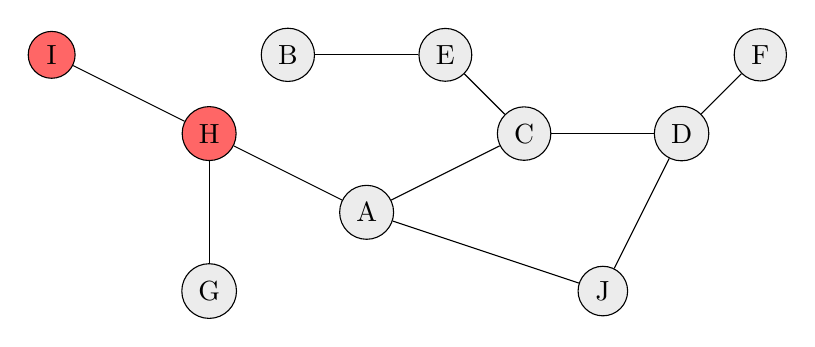
\begin{tikzpicture}
\node[draw,circle,fill=gray!15] (A)at(0,0) {A};
\node[draw,circle,fill=gray!15] (B)at(-1,2) {B};
\node[draw,circle,fill=gray!15] (C)at(2,1) {C};
\node[draw,circle,fill=gray!15] (D)at(4,1) {D};
\node[draw,circle,fill=gray!15] (E)at(1,2) {E};
\node[draw,circle,fill=gray!15] (F)at(5,2) {F};
\node[draw,circle,fill=gray!15] (G)at(-2,-1) {G};
\node[draw,circle,fill=red!60] (H)at(-2,1) {H};
\node[draw,circle,fill=red!60] (I)at(-4,2) {I};
\node[draw,circle,fill=gray!15] (J)at(3,-1) {J};
\draw[-,>=latex] (E) -- (B);
\draw[-,>=latex] (A) -- (C);
\draw[-,>=latex] (A) -- (H);
\draw[-,>=latex] (A) -- (J);
\draw[-,>=latex] (H) -- (I);
\draw[-,>=latex] (H) -- (G);
\draw[-,>=latex] (C) -- (E);
\draw[-,>=latex] (C) -- (D);
%\draw[-,>=latex] (C) -- (J);
\draw[-,>=latex] (D) -- (J);
\draw[-,>=latex] (D) -- (F);
\end{tikzpicture}
\end{center}
\begin{center}
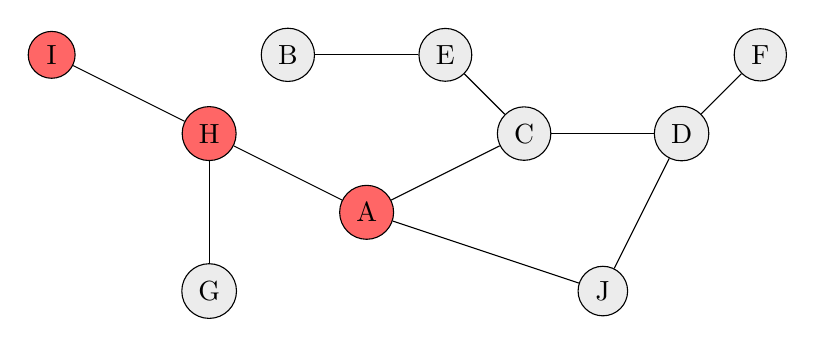
\begin{tikzpicture}
\node[draw,circle,fill=red!60] (A)at(0,0) {A};
\node[draw,circle,fill=gray!15] (B)at(-1,2) {B};
\node[draw,circle,fill=gray!15] (C)at(2,1) {C};
\node[draw,circle,fill=gray!15] (D)at(4,1) {D};
\node[draw,circle,fill=gray!15] (E)at(1,2) {E};
\node[draw,circle,fill=gray!15] (F)at(5,2) {F};
\node[draw,circle,fill=gray!15] (G)at(-2,-1) {G};
\node[draw,circle,fill=red!60] (H)at(-2,1) {H};
\node[draw,circle,fill=red!60] (I)at(-4,2) {I};
\node[draw,circle,fill=gray!15] (J)at(3,-1) {J};
\draw[-,>=latex] (E) -- (B);
\draw[-,>=latex] (A) -- (C);
\draw[-,>=latex] (A) -- (H);
\draw[-,>=latex] (A) -- (J);
\draw[-,>=latex] (H) -- (I);
\draw[-,>=latex] (H) -- (G);
\draw[-,>=latex] (C) -- (E);
\draw[-,>=latex] (C) -- (D);
%\draw[-,>=latex] (C) -- (J);
\draw[-,>=latex] (D) -- (J);
\draw[-,>=latex] (D) -- (F);
\end{tikzpicture}
\end{center}
\begin{center}
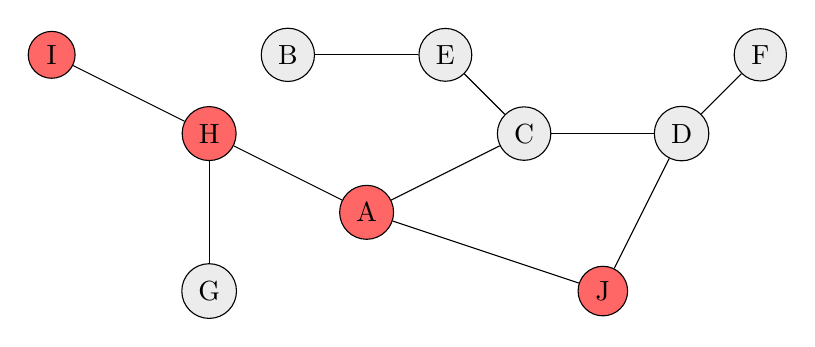
\begin{tikzpicture}
\node[draw,circle,fill=red!60] (A)at(0,0) {A};
\node[draw,circle,fill=gray!15] (B)at(-1,2) {B};
\node[draw,circle,fill=gray!15] (C)at(2,1) {C};
\node[draw,circle,fill=gray!15] (D)at(4,1) {D};
\node[draw,circle,fill=gray!15] (E)at(1,2) {E};
\node[draw,circle,fill=gray!15] (F)at(5,2) {F};
\node[draw,circle,fill=gray!15] (G)at(-2,-1) {G};
\node[draw,circle,fill=red!60] (H)at(-2,1) {H};
\node[draw,circle,fill=red!60] (I)at(-4,2) {I};
\node[draw,circle,fill=red!60] (J)at(3,-1) {J};
\draw[-,>=latex] (E) -- (B);
\draw[-,>=latex] (A) -- (C);
\draw[-,>=latex] (A) -- (H);
\draw[-,>=latex] (A) -- (J);
\draw[-,>=latex] (H) -- (I);
\draw[-,>=latex] (H) -- (G);
\draw[-,>=latex] (C) -- (E);
\draw[-,>=latex] (C) -- (D);
%\draw[-,>=latex] (C) -- (J);
\draw[-,>=latex] (D) -- (J);
\draw[-,>=latex] (D) -- (F);
\end{tikzpicture}
\end{center}
\begin{center}
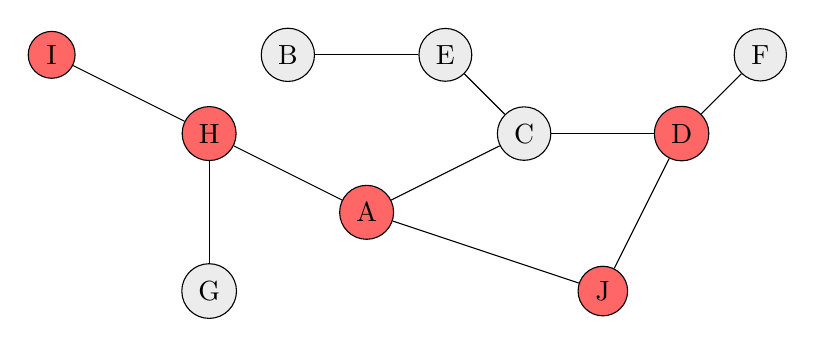
\begin{tikzpicture}
\node[draw,circle,fill=red!60] (A)at(0,0) {A};
\node[draw,circle,fill=gray!15] (B)at(-1,2) {B};
\node[draw,circle,fill=gray!15] (C)at(2,1) {C};
\node[draw,circle,fill=red!60] (D)at(4,1) {D};
\node[draw,circle,fill=gray!15] (E)at(1,2) {E};
\node[draw,circle,fill=gray!15] (F)at(5,2) {F};
\node[draw,circle,fill=gray!15] (G)at(-2,-1) {G};
\node[draw,circle,fill=red!60] (H)at(-2,1) {H};
\node[draw,circle,fill=red!60] (I)at(-4,2) {I};
\node[draw,circle,fill=red!60] (J)at(3,-1) {J};
\draw[-,>=latex] (E) -- (B);
\draw[-,>=latex] (A) -- (C);
\draw[-,>=latex] (A) -- (H);
\draw[-,>=latex] (A) -- (J);
\draw[-,>=latex] (H) -- (I);
\draw[-,>=latex] (H) -- (G);
\draw[-,>=latex] (C) -- (E);
\draw[-,>=latex] (C) -- (D);
%\draw[-,>=latex] (C) -- (J);
\draw[-,>=latex] (D) -- (J);
\draw[-,>=latex] (D) -- (F);
\end{tikzpicture}
\end{center}
\begin{center}
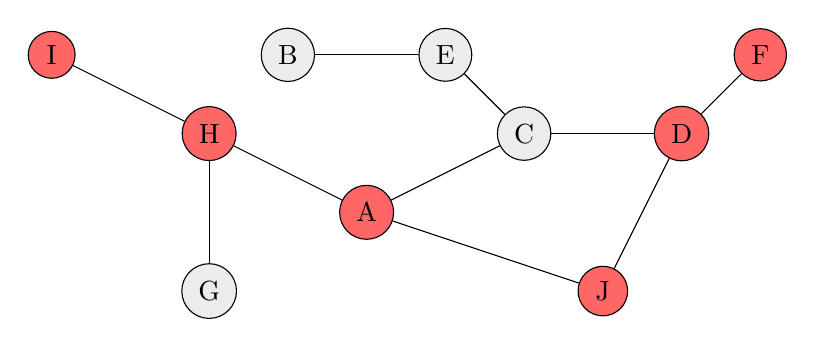
\begin{tikzpicture}
\node[draw,circle,fill=red!60] (A)at(0,0) {A};
\node[draw,circle,fill=gray!15] (B)at(-1,2) {B};
\node[draw,circle,fill=gray!15] (C)at(2,1) {C};
\node[draw,circle,fill=red!60] (D)at(4,1) {D};
\node[draw,circle,fill=gray!15] (E)at(1,2) {E};
\node[draw,circle,fill=red!60] (F)at(5,2) {F};
\node[draw,circle,fill=gray!15] (G)at(-2,-1) {G};
\node[draw,circle,fill=red!60] (H)at(-2,1) {H};
\node[draw,circle,fill=red!60] (I)at(-4,2) {I};
\node[draw,circle,fill=red!60] (J)at(3,-1) {J};
\draw[-,>=latex] (E) -- (B);
\draw[-,>=latex] (A) -- (C);
\draw[-,>=latex] (A) -- (H);
\draw[-,>=latex] (A) -- (J);
\draw[-,>=latex] (H) -- (I);
\draw[-,>=latex] (H) -- (G);
\draw[-,>=latex] (C) -- (E);
\draw[-,>=latex] (C) -- (D);
%\draw[-,>=latex] (C) -- (J);
\draw[-,>=latex] (D) -- (J);
\draw[-,>=latex] (D) -- (F);
\end{tikzpicture}
\end{center}
\begin{center}
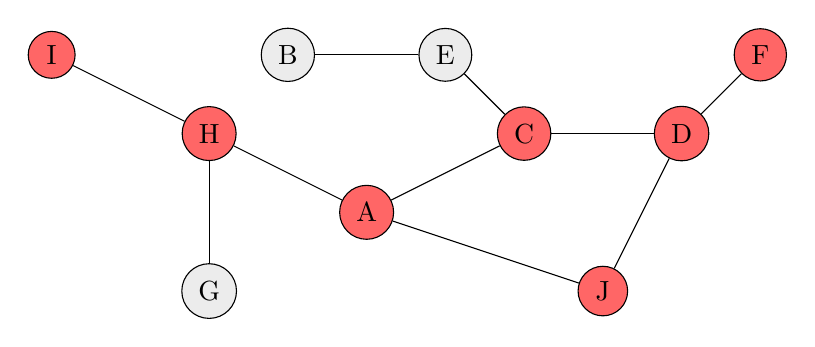
\begin{tikzpicture}
\node[draw,circle,fill=red!60] (A)at(0,0) {A};
\node[draw,circle,fill=gray!15] (B)at(-1,2) {B};
\node[draw,circle,fill=red!60] (C)at(2,1) {C};
\node[draw,circle,fill=red!60] (D)at(4,1) {D};
\node[draw,circle,fill=gray!15] (E)at(1,2) {E};
\node[draw,circle,fill=red!60] (F)at(5,2) {F};
\node[draw,circle,fill=gray!15] (G)at(-2,-1) {G};
\node[draw,circle,fill=red!60] (H)at(-2,1) {H};
\node[draw,circle,fill=red!60] (I)at(-4,2) {I};
\node[draw,circle,fill=red!60] (J)at(3,-1) {J};
\draw[-,>=latex] (E) -- (B);
\draw[-,>=latex] (A) -- (C);
\draw[-,>=latex] (A) -- (H);
\draw[-,>=latex] (A) -- (J);
\draw[-,>=latex] (H) -- (I);
\draw[-,>=latex] (H) -- (G);
\draw[-,>=latex] (C) -- (E);
\draw[-,>=latex] (C) -- (D);
%\draw[-,>=latex] (C) -- (J);
\draw[-,>=latex] (D) -- (J);
\draw[-,>=latex] (D) -- (F);
\end{tikzpicture}
\end{center}
\begin{center}
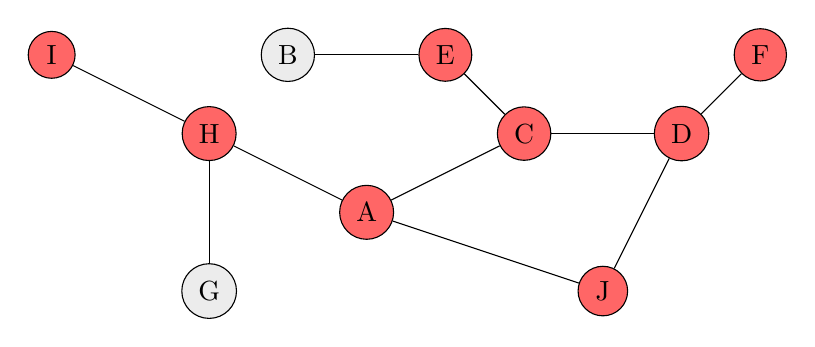
\begin{tikzpicture}
\node[draw,circle,fill=red!60] (A)at(0,0) {A};
\node[draw,circle,fill=gray!15] (B)at(-1,2) {B};
\node[draw,circle,fill=red!60] (C)at(2,1) {C};
\node[draw,circle,fill=red!60] (D)at(4,1) {D};
\node[draw,circle,fill=red!60] (E)at(1,2) {E};
\node[draw,circle,fill=red!60] (F)at(5,2) {F};
\node[draw,circle,fill=gray!15] (G)at(-2,-1) {G};
\node[draw,circle,fill=red!60] (H)at(-2,1) {H};
\node[draw,circle,fill=red!60] (I)at(-4,2) {I};
\node[draw,circle,fill=red!60] (J)at(3,-1) {J};
\draw[-,>=latex] (E) -- (B);
\draw[-,>=latex] (A) -- (C);
\draw[-,>=latex] (A) -- (H);
\draw[-,>=latex] (A) -- (J);
\draw[-,>=latex] (H) -- (I);
\draw[-,>=latex] (H) -- (G);
\draw[-,>=latex] (C) -- (E);
\draw[-,>=latex] (C) -- (D);
%\draw[-,>=latex] (C) -- (J);
\draw[-,>=latex] (D) -- (J);
\draw[-,>=latex] (D) -- (F);
\end{tikzpicture}
\end{center}
\begin{center}
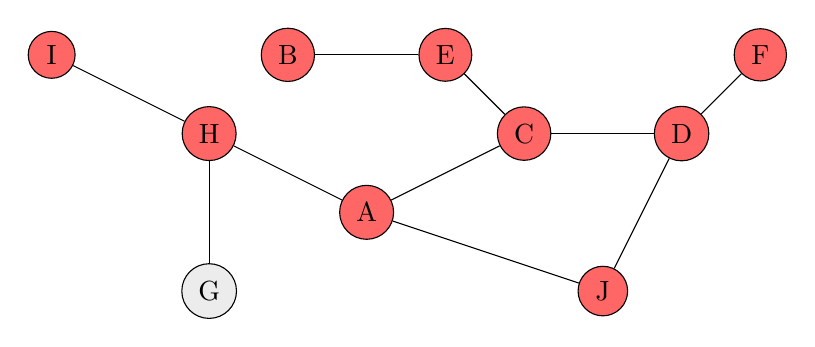
\begin{tikzpicture}
\node[draw,circle,fill=red!60] (A)at(0,0) {A};
\node[draw,circle,fill=red!60] (B)at(-1,2) {B};
\node[draw,circle,fill=red!60] (C)at(2,1) {C};
\node[draw,circle,fill=red!60] (D)at(4,1) {D};
\node[draw,circle,fill=red!60] (E)at(1,2) {E};
\node[draw,circle,fill=red!60] (F)at(5,2) {F};
\node[draw,circle,fill=gray!15] (G)at(-2,-1) {G};
\node[draw,circle,fill=red!60] (H)at(-2,1) {H};
\node[draw,circle,fill=red!60] (I)at(-4,2) {I};
\node[draw,circle,fill=red!60] (J)at(3,-1) {J};
\draw[-,>=latex] (E) -- (B);
\draw[-,>=latex] (A) -- (C);
\draw[-,>=latex] (A) -- (H);
\draw[-,>=latex] (A) -- (J);
\draw[-,>=latex] (H) -- (I);
\draw[-,>=latex] (H) -- (G);
\draw[-,>=latex] (C) -- (E);
\draw[-,>=latex] (C) -- (D);
%\draw[-,>=latex] (C) -- (J);
\draw[-,>=latex] (D) -- (J);
\draw[-,>=latex] (D) -- (F);
\end{tikzpicture}
\end{center}
\begin{center}
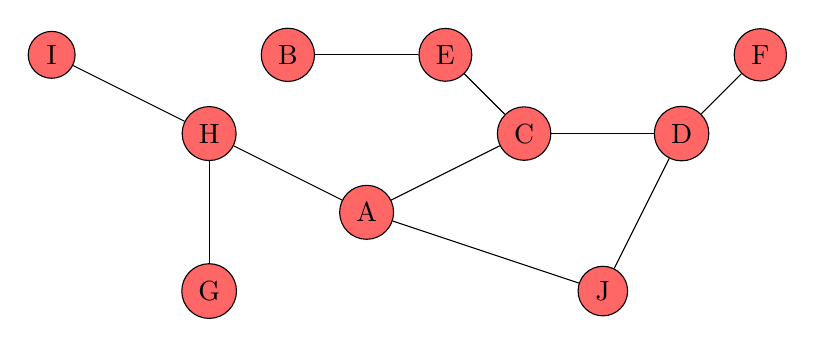
\begin{tikzpicture}
\node[draw,circle,fill=red!60] (A)at(0,0) {A};
\node[draw,circle,fill=red!60] (B)at(-1,2) {B};
\node[draw,circle,fill=red!60] (C)at(2,1) {C};
\node[draw,circle,fill=red!60] (D)at(4,1) {D};
\node[draw,circle,fill=red!60] (E)at(1,2) {E};
\node[draw,circle,fill=red!60] (F)at(5,2) {F};
\node[draw,circle,fill=red!60] (G)at(-2,-1) {G};
\node[draw,circle,fill=red!60] (H)at(-2,1) {H};
\node[draw,circle,fill=red!60] (I)at(-4,2) {I};
\node[draw,circle,fill=red!60] (J)at(3,-1) {J};
\draw[-,>=latex] (E) -- (B);
\draw[-,>=latex] (A) -- (C);
\draw[-,>=latex] (A) -- (H);
\draw[-,>=latex] (A) -- (J);
\draw[-,>=latex] (H) -- (I);
\draw[-,>=latex] (H) -- (G);
\draw[-,>=latex] (C) -- (E);
\draw[-,>=latex] (C) -- (D);
%\draw[-,>=latex] (C) -- (J);
\draw[-,>=latex] (D) -- (J);
\draw[-,>=latex] (D) -- (F);
\end{tikzpicture}
\end{center}
\pagebreak
DFS
\begin{center}
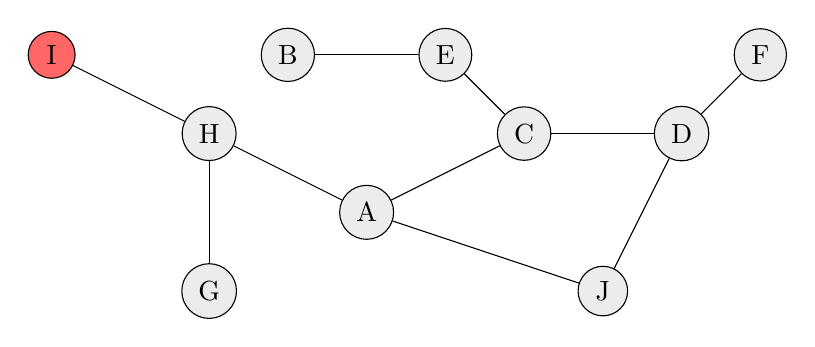
\begin{tikzpicture}
\node[draw,circle,fill=gray!15] (A)at(0,0) {A};
\node[draw,circle,fill=gray!15] (B)at(-1,2) {B};
\node[draw,circle,fill=gray!15] (C)at(2,1) {C};
\node[draw,circle,fill=gray!15] (D)at(4,1) {D};
\node[draw,circle,fill=gray!15] (E)at(1,2) {E};
\node[draw,circle,fill=gray!15] (F)at(5,2) {F};
\node[draw,circle,fill=gray!15] (G)at(-2,-1) {G};
\node[draw,circle,fill=gray!15] (H)at(-2,1) {H};
\node[draw,circle,fill=red!60] (I)at(-4,2) {I};
\node[draw,circle,fill=gray!15] (J)at(3,-1) {J};
\draw[-,>=latex] (E) -- (B);
\draw[-,>=latex] (A) -- (C);
\draw[-,>=latex] (A) -- (H);
\draw[-,>=latex] (A) -- (J);
\draw[-,>=latex] (H) -- (I);
\draw[-,>=latex] (H) -- (G);
\draw[-,>=latex] (C) -- (E);
\draw[-,>=latex] (C) -- (D);
%\draw[-,>=latex] (C) -- (J);
\draw[-,>=latex] (D) -- (J);
\draw[-,>=latex] (D) -- (F);
\end{tikzpicture}
\end{center}

\begin{center}
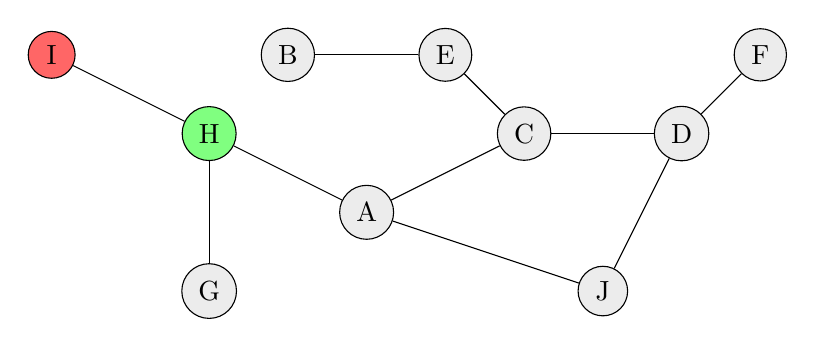
\begin{tikzpicture}
\node[draw,circle,fill=gray!15] (A)at(0,0) {A};
\node[draw,circle,fill=gray!15] (B)at(-1,2) {B};
\node[draw,circle,fill=gray!15] (C)at(2,1) {C};
\node[draw,circle,fill=gray!15] (D)at(4,1) {D};
\node[draw,circle,fill=gray!15] (E)at(1,2) {E};
\node[draw,circle,fill=gray!15] (F)at(5,2) {F};
\node[draw,circle,fill=gray!15] (G)at(-2,-1) {G};
\node[draw,circle,fill=green!50] (H)at(-2,1) {H};
\node[draw,circle,fill=red!60] (I)at(-4,2) {I};
\node[draw,circle,fill=gray!15] (J)at(3,-1) {J};
\draw[-,>=latex] (E) -- (B);
\draw[-,>=latex] (A) -- (C);
\draw[-,>=latex] (A) -- (H);
\draw[-,>=latex] (A) -- (J);
\draw[-,>=latex] (H) -- (I);
\draw[-,>=latex] (H) -- (G);
\draw[-,>=latex] (C) -- (E);
\draw[-,>=latex] (C) -- (D);
%\draw[-,>=latex] (C) -- (J);
\draw[-,>=latex] (D) -- (J);
\draw[-,>=latex] (D) -- (F);
\end{tikzpicture}
\end{center}

\begin{center}
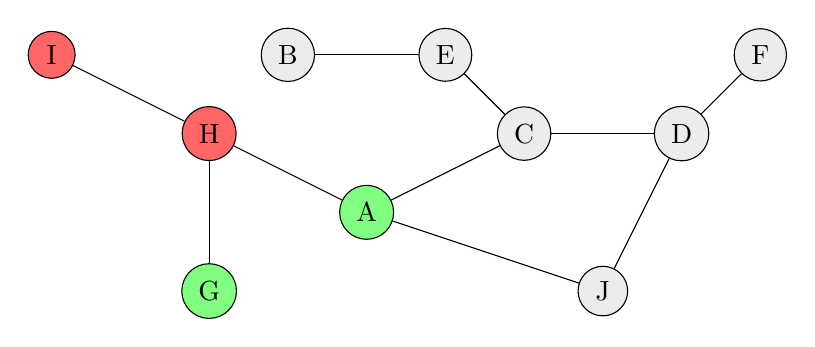
\begin{tikzpicture}
\node[draw,circle,fill=green!50] (A)at(0,0) {A};
\node[draw,circle,fill=gray!15] (B)at(-1,2) {B};
\node[draw,circle,fill=gray!15] (C)at(2,1) {C};
\node[draw,circle,fill=gray!15] (D)at(4,1) {D};
\node[draw,circle,fill=gray!15] (E)at(1,2) {E};
\node[draw,circle,fill=gray!15] (F)at(5,2) {F};
\node[draw,circle,fill=green!50] (G)at(-2,-1) {G};
\node[draw,circle,fill=red!60] (H)at(-2,1) {H};
\node[draw,circle,fill=red!60] (I)at(-4,2) {I};
\node[draw,circle,fill=gray!15] (J)at(3,-1) {J};
\draw[-,>=latex] (E) -- (B);
\draw[-,>=latex] (A) -- (C);
\draw[-,>=latex] (A) -- (H);
\draw[-,>=latex] (A) -- (J);
\draw[-,>=latex] (H) -- (I);
\draw[-,>=latex] (H) -- (G);
\draw[-,>=latex] (C) -- (E);
\draw[-,>=latex] (C) -- (D);
%\draw[-,>=latex] (C) -- (J);
\draw[-,>=latex] (D) -- (J);
\draw[-,>=latex] (D) -- (F);
\end{tikzpicture}
\end{center}

\begin{center}
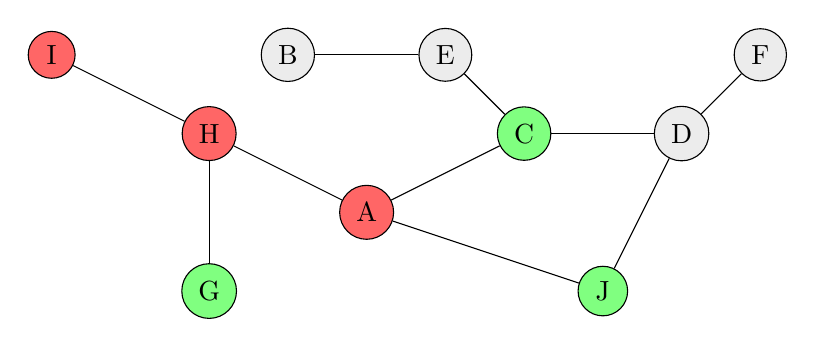
\begin{tikzpicture}
\node[draw,circle,fill=red!60] (A)at(0,0) {A};
\node[draw,circle,fill=gray!15] (B)at(-1,2) {B};
\node[draw,circle,fill=green!50] (C)at(2,1) {C};
\node[draw,circle,fill=gray!15] (D)at(4,1) {D};
\node[draw,circle,fill=gray!15] (E)at(1,2) {E};
\node[draw,circle,fill=gray!15] (F)at(5,2) {F};
\node[draw,circle,fill=green!50] (G)at(-2,-1) {G};
\node[draw,circle,fill=red!60] (H)at(-2,1) {H};
\node[draw,circle,fill=red!60] (I)at(-4,2) {I};
\node[draw,circle,fill=green!50] (J)at(3,-1) {J};
\draw[-,>=latex] (E) -- (B);
\draw[-,>=latex] (A) -- (C);
\draw[-,>=latex] (A) -- (H);
\draw[-,>=latex] (A) -- (J);
\draw[-,>=latex] (H) -- (I);
\draw[-,>=latex] (H) -- (G);
\draw[-,>=latex] (C) -- (E);
\draw[-,>=latex] (C) -- (D);
%\draw[-,>=latex] (C) -- (J);
\draw[-,>=latex] (D) -- (J);
\draw[-,>=latex] (D) -- (F);
\end{tikzpicture}
\end{center}

\begin{center}
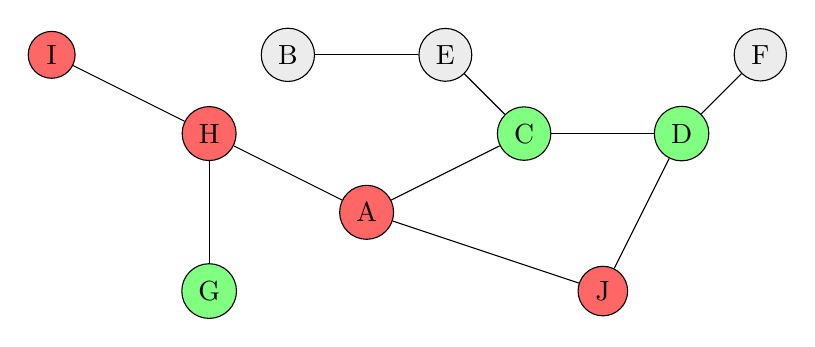
\begin{tikzpicture}
\node[draw,circle,fill=red!60] (A)at(0,0) {A};
\node[draw,circle,fill=gray!15] (B)at(-1,2) {B};
\node[draw,circle,fill=green!50] (C)at(2,1) {C};
\node[draw,circle,fill=green!50] (D)at(4,1) {D};
\node[draw,circle,fill=gray!15] (E)at(1,2) {E};
\node[draw,circle,fill=gray!15] (F)at(5,2) {F};
\node[draw,circle,fill=green!50] (G)at(-2,-1) {G};
\node[draw,circle,fill=red!60] (H)at(-2,1) {H};
\node[draw,circle,fill=red!60] (I)at(-4,2) {I};
\node[draw,circle,fill=red!60] (J)at(3,-1) {J};
\draw[-,>=latex] (E) -- (B);
\draw[-,>=latex] (A) -- (C);
\draw[-,>=latex] (A) -- (H);
\draw[-,>=latex] (A) -- (J);
\draw[-,>=latex] (H) -- (I);
\draw[-,>=latex] (H) -- (G);
\draw[-,>=latex] (C) -- (E);
\draw[-,>=latex] (C) -- (D);
%\draw[-,>=latex] (C) -- (J);
\draw[-,>=latex] (D) -- (J);
\draw[-,>=latex] (D) -- (F);
\end{tikzpicture}
\end{center}

\begin{center}
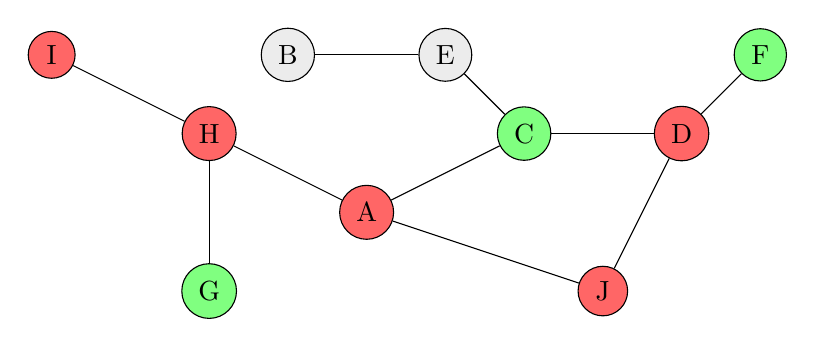
\begin{tikzpicture}
\node[draw,circle,fill=red!60] (A)at(0,0) {A};
\node[draw,circle,fill=gray!15] (B)at(-1,2) {B};
\node[draw,circle,fill=green!50] (C)at(2,1) {C};
\node[draw,circle,fill=red!60] (D)at(4,1) {D};
\node[draw,circle,fill=gray!15] (E)at(1,2) {E};
\node[draw,circle,fill=green!50] (F)at(5,2) {F};
\node[draw,circle,fill=green!50] (G)at(-2,-1) {G};
\node[draw,circle,fill=red!60] (H)at(-2,1) {H};
\node[draw,circle,fill=red!60] (I)at(-4,2) {I};
\node[draw,circle,fill=red!60] (J)at(3,-1) {J};
\draw[-,>=latex] (E) -- (B);
\draw[-,>=latex] (A) -- (C);
\draw[-,>=latex] (A) -- (H);
\draw[-,>=latex] (A) -- (J);
\draw[-,>=latex] (H) -- (I);
\draw[-,>=latex] (H) -- (G);
\draw[-,>=latex] (C) -- (E);
\draw[-,>=latex] (C) -- (D);
%\draw[-,>=latex] (C) -- (J);
\draw[-,>=latex] (D) -- (J);
\draw[-,>=latex] (D) -- (F);
\end{tikzpicture}
\end{center}

\begin{center}
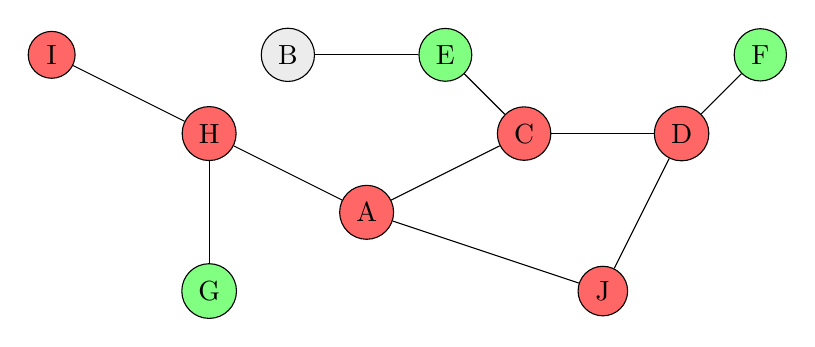
\begin{tikzpicture}
\node[draw,circle,fill=red!60] (A)at(0,0) {A};
\node[draw,circle,fill=gray!15] (B)at(-1,2) {B};
\node[draw,circle,fill=red!60] (C)at(2,1) {C};
\node[draw,circle,fill=red!60] (D)at(4,1) {D};
\node[draw,circle,fill=green!50] (E)at(1,2) {E};
\node[draw,circle,fill=green!50] (F)at(5,2) {F};
\node[draw,circle,fill=green!50] (G)at(-2,-1) {G};
\node[draw,circle,fill=red!60] (H)at(-2,1) {H};
\node[draw,circle,fill=red!60] (I)at(-4,2) {I};
\node[draw,circle,fill=red!60] (J)at(3,-1) {J};
\draw[-,>=latex] (E) -- (B);
\draw[-,>=latex] (A) -- (C);
\draw[-,>=latex] (A) -- (H);
\draw[-,>=latex] (A) -- (J);
\draw[-,>=latex] (H) -- (I);
\draw[-,>=latex] (H) -- (G);
\draw[-,>=latex] (C) -- (E);
\draw[-,>=latex] (C) -- (D);
%\draw[-,>=latex] (C) -- (J);
\draw[-,>=latex] (D) -- (J);
\draw[-,>=latex] (D) -- (F);
\end{tikzpicture}
\end{center}

\begin{center}
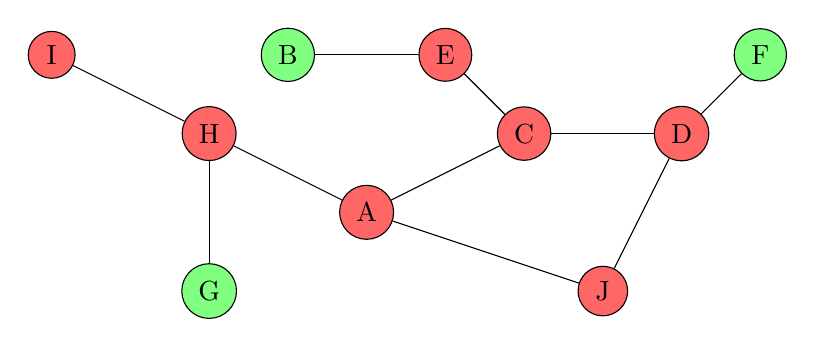
\begin{tikzpicture}
\node[draw,circle,fill=red!60] (A)at(0,0) {A};
\node[draw,circle,fill=green!50] (B)at(-1,2) {B};
\node[draw,circle,fill=red!60] (C)at(2,1) {C};
\node[draw,circle,fill=red!60] (D)at(4,1) {D};
\node[draw,circle,fill=red!60] (E)at(1,2) {E};
\node[draw,circle,fill=green!50] (F)at(5,2) {F};
\node[draw,circle,fill=green!50] (G)at(-2,-1) {G};
\node[draw,circle,fill=red!60] (H)at(-2,1) {H};
\node[draw,circle,fill=red!60] (I)at(-4,2) {I};
\node[draw,circle,fill=red!60] (J)at(3,-1) {J};
\draw[-,>=latex] (E) -- (B);
\draw[-,>=latex] (A) -- (C);
\draw[-,>=latex] (A) -- (H);
\draw[-,>=latex] (A) -- (J);
\draw[-,>=latex] (H) -- (I);
\draw[-,>=latex] (H) -- (G);
\draw[-,>=latex] (C) -- (E);
\draw[-,>=latex] (C) -- (D);
%\draw[-,>=latex] (C) -- (J);
\draw[-,>=latex] (D) -- (J);
\draw[-,>=latex] (D) -- (F);
\end{tikzpicture}
\end{center}

\begin{center}
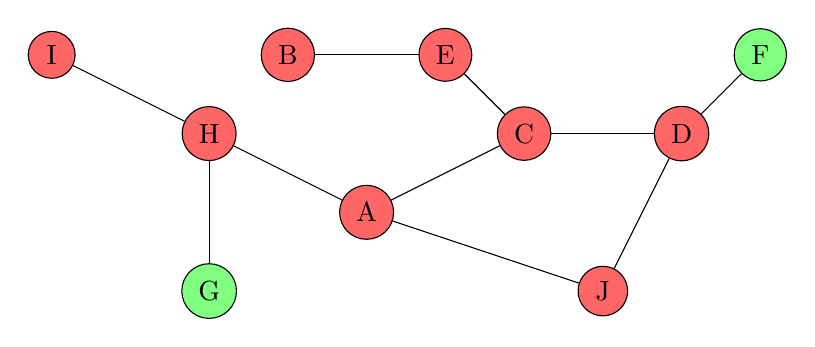
\begin{tikzpicture}
\node[draw,circle,fill=red!60] (A)at(0,0) {A};
\node[draw,circle,fill=red!60] (B)at(-1,2) {B};
\node[draw,circle,fill=red!60] (C)at(2,1) {C};
\node[draw,circle,fill=red!60] (D)at(4,1) {D};
\node[draw,circle,fill=red!60] (E)at(1,2) {E};
\node[draw,circle,fill=green!50] (F)at(5,2) {F};
\node[draw,circle,fill=green!50] (G)at(-2,-1) {G};
\node[draw,circle,fill=red!60] (H)at(-2,1) {H};
\node[draw,circle,fill=red!60] (I)at(-4,2) {I};
\node[draw,circle,fill=red!60] (J)at(3,-1) {J};
\draw[-,>=latex] (E) -- (B);
\draw[-,>=latex] (A) -- (C);
\draw[-,>=latex] (A) -- (H);
\draw[-,>=latex] (A) -- (J);
\draw[-,>=latex] (H) -- (I);
\draw[-,>=latex] (H) -- (G);
\draw[-,>=latex] (C) -- (E);
\draw[-,>=latex] (C) -- (D);
%\draw[-,>=latex] (C) -- (J);
\draw[-,>=latex] (D) -- (J);
\draw[-,>=latex] (D) -- (F);
\end{tikzpicture}
\end{center}

\begin{center}
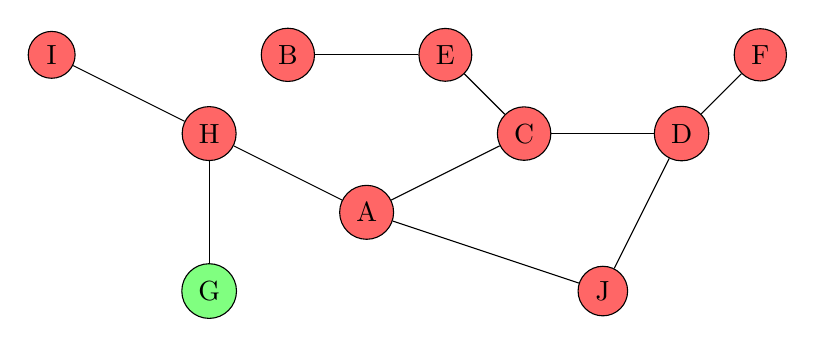
\begin{tikzpicture}
\node[draw,circle,fill=red!60] (A)at(0,0) {A};
\node[draw,circle,fill=red!60] (B)at(-1,2) {B};
\node[draw,circle,fill=red!60] (C)at(2,1) {C};
\node[draw,circle,fill=red!60] (D)at(4,1) {D};
\node[draw,circle,fill=red!60] (E)at(1,2) {E};
\node[draw,circle,fill=red!60] (F)at(5,2) {F};
\node[draw,circle,fill=green!50] (G)at(-2,-1) {G};
\node[draw,circle,fill=red!60] (H)at(-2,1) {H};
\node[draw,circle,fill=red!60] (I)at(-4,2) {I};
\node[draw,circle,fill=red!60] (J)at(3,-1) {J};
\draw[-,>=latex] (E) -- (B);
\draw[-,>=latex] (A) -- (C);
\draw[-,>=latex] (A) -- (H);
\draw[-,>=latex] (A) -- (J);
\draw[-,>=latex] (H) -- (I);
\draw[-,>=latex] (H) -- (G);
\draw[-,>=latex] (C) -- (E);
\draw[-,>=latex] (C) -- (D);
%\draw[-,>=latex] (C) -- (J);
\draw[-,>=latex] (D) -- (J);
\draw[-,>=latex] (D) -- (F);
\end{tikzpicture}
\end{center}

\begin{center}
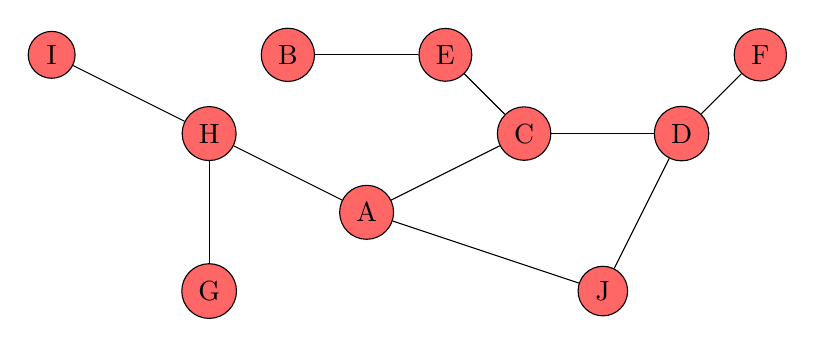
\begin{tikzpicture}
\node[draw,circle,fill=red!60] (A)at(0,0) {A};
\node[draw,circle,fill=red!60] (B)at(-1,2) {B};
\node[draw,circle,fill=red!60] (C)at(2,1) {C};
\node[draw,circle,fill=red!60] (D)at(4,1) {D};
\node[draw,circle,fill=red!60] (E)at(1,2) {E};
\node[draw,circle,fill=red!60] (F)at(5,2) {F};
\node[draw,circle,fill=red!60] (G)at(-2,-1) {G};
\node[draw,circle,fill=red!60] (H)at(-2,1) {H};
\node[draw,circle,fill=red!60] (I)at(-4,2) {I};
\node[draw,circle,fill=red!60] (J)at(3,-1) {J};
\draw[-,>=latex] (E) -- (B);
\draw[-,>=latex] (A) -- (C);
\draw[-,>=latex] (A) -- (H);
\draw[-,>=latex] (A) -- (J);
\draw[-,>=latex] (H) -- (I);
\draw[-,>=latex] (H) -- (G);
\draw[-,>=latex] (C) -- (E);
\draw[-,>=latex] (C) -- (D);
%\draw[-,>=latex] (C) -- (J);
\draw[-,>=latex] (D) -- (J);
\draw[-,>=latex] (D) -- (F);
\end{tikzpicture}
\end{center}
\pagebreak
BFS à la main
\begin{center}
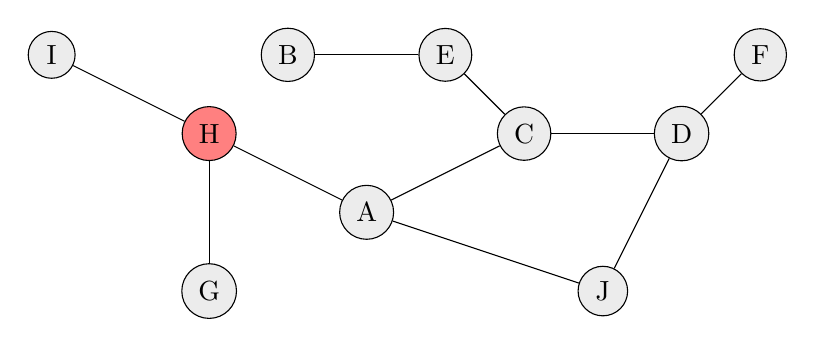
\begin{tikzpicture}
\node[draw,circle,fill=gray!15] (A)at(0,0) {A};
\node[draw,circle,fill=gray!15] (B)at(-1,2) {B};
\node[draw,circle,fill=gray!15] (C)at(2,1) {C};
\node[draw,circle,fill=gray!15] (D)at(4,1) {D};
\node[draw,circle,fill=gray!15] (E)at(1,2) {E};
\node[draw,circle,fill=gray!15] (F)at(5,2) {F};
\node[draw,circle,fill=gray!15] (G)at(-2,-1) {G};
\node[draw,circle,fill=red!50] (H)at(-2,1) {H};
\node[draw,circle,fill=gray!15] (I)at(-4,2) {I};
\node[draw,circle,fill=gray!15] (J)at(3,-1) {J};
\draw[-,>=latex] (E) -- (B);
\draw[-,>=latex] (A) -- (C);
\draw[-,>=latex] (A) -- (H);
\draw[-,>=latex] (A) -- (J);
\draw[-,>=latex] (H) -- (I);
\draw[-,>=latex] (H) -- (G);
\draw[-,>=latex] (C) -- (E);
\draw[-,>=latex] (C) -- (D);
%\draw[-,>=latex] (C) -- (J);
\draw[-,>=latex] (D) -- (J);
\draw[-,>=latex] (D) -- (F);
\end{tikzpicture}
\end{center}

\begin{center}
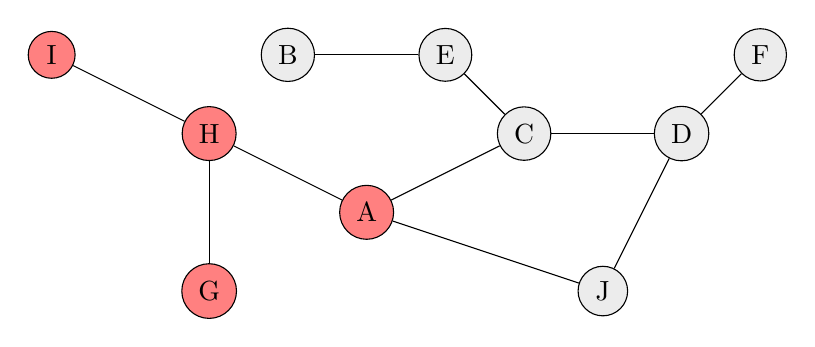
\begin{tikzpicture}
\node[draw,circle,fill=red!50] (A)at(0,0) {A};
\node[draw,circle,fill=gray!15] (B)at(-1,2) {B};
\node[draw,circle,fill=gray!15] (C)at(2,1) {C};
\node[draw,circle,fill=gray!15] (D)at(4,1) {D};
\node[draw,circle,fill=gray!15] (E)at(1,2) {E};
\node[draw,circle,fill=gray!15] (F)at(5,2) {F};
\node[draw,circle,fill=red!50] (G)at(-2,-1) {G};
\node[draw,circle,fill=red!50] (H)at(-2,1) {H};
\node[draw,circle,fill=red!50] (I)at(-4,2) {I};
\node[draw,circle,fill=gray!15] (J)at(3,-1) {J};
\draw[-,>=latex] (E) -- (B);
\draw[-,>=latex] (A) -- (C);
\draw[-,>=latex] (A) -- (H);
\draw[-,>=latex] (A) -- (J);
\draw[-,>=latex] (H) -- (I);
\draw[-,>=latex] (H) -- (G);
\draw[-,>=latex] (C) -- (E);
\draw[-,>=latex] (C) -- (D);
%\draw[-,>=latex] (C) -- (J);
\draw[-,>=latex] (D) -- (J);
\draw[-,>=latex] (D) -- (F);
\end{tikzpicture}
\end{center}

\begin{center}
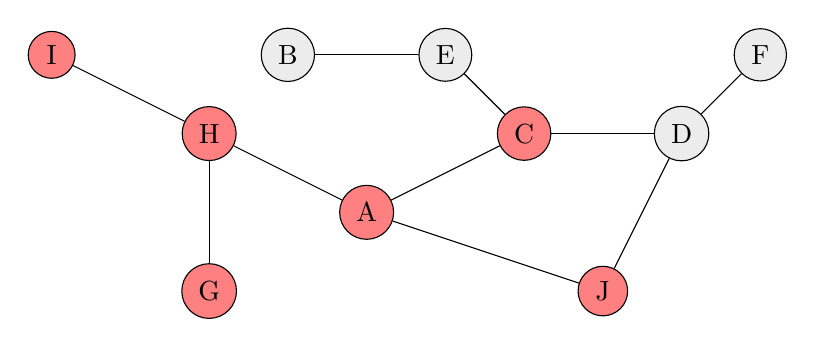
\begin{tikzpicture}
\node[draw,circle,fill=red!50] (A)at(0,0) {A};
\node[draw,circle,fill=gray!15] (B)at(-1,2) {B};
\node[draw,circle,fill=red!50] (C)at(2,1) {C};
\node[draw,circle,fill=gray!15] (D)at(4,1) {D};
\node[draw,circle,fill=gray!15] (E)at(1,2) {E};
\node[draw,circle,fill=gray!15] (F)at(5,2) {F};
\node[draw,circle,fill=red!50] (G)at(-2,-1) {G};
\node[draw,circle,fill=red!50] (H)at(-2,1) {H};
\node[draw,circle,fill=red!50] (I)at(-4,2) {I};
\node[draw,circle,fill=red!50] (J)at(3,-1) {J};
\draw[-,>=latex] (E) -- (B);
\draw[-,>=latex] (A) -- (C);
\draw[-,>=latex] (A) -- (H);
\draw[-,>=latex] (A) -- (J);
\draw[-,>=latex] (H) -- (I);
\draw[-,>=latex] (H) -- (G);
\draw[-,>=latex] (C) -- (E);
\draw[-,>=latex] (C) -- (D);
%\draw[-,>=latex] (C) -- (J);
\draw[-,>=latex] (D) -- (J);
\draw[-,>=latex] (D) -- (F);
\end{tikzpicture}
\end{center}

\begin{center}
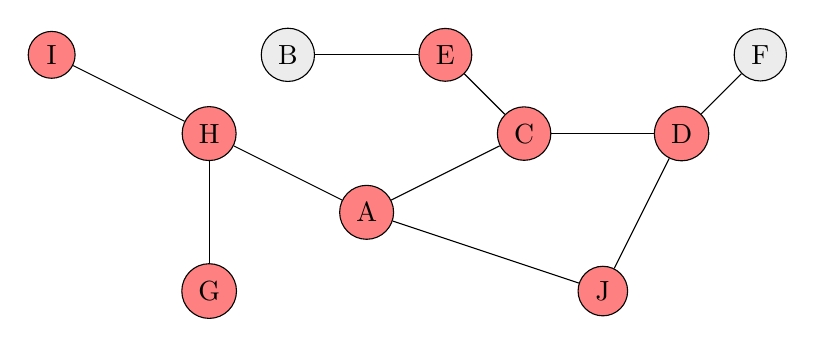
\begin{tikzpicture}
\node[draw,circle,fill=red!50] (A)at(0,0) {A};
\node[draw,circle,fill=gray!15] (B)at(-1,2) {B};
\node[draw,circle,fill=red!50] (C)at(2,1) {C};
\node[draw,circle,fill=red!50] (D)at(4,1) {D};
\node[draw,circle,fill=red!50] (E)at(1,2) {E};
\node[draw,circle,fill=gray!15] (F)at(5,2) {F};
\node[draw,circle,fill=red!50] (G)at(-2,-1) {G};
\node[draw,circle,fill=red!50] (H)at(-2,1) {H};
\node[draw,circle,fill=red!50] (I)at(-4,2) {I};
\node[draw,circle,fill=red!50] (J)at(3,-1) {J};
\draw[-,>=latex] (E) -- (B);
\draw[-,>=latex] (A) -- (C);
\draw[-,>=latex] (A) -- (H);
\draw[-,>=latex] (A) -- (J);
\draw[-,>=latex] (H) -- (I);
\draw[-,>=latex] (H) -- (G);
\draw[-,>=latex] (C) -- (E);
\draw[-,>=latex] (C) -- (D);
%\draw[-,>=latex] (C) -- (J);
\draw[-,>=latex] (D) -- (J);
\draw[-,>=latex] (D) -- (F);
\end{tikzpicture}
\end{center}

\begin{center}
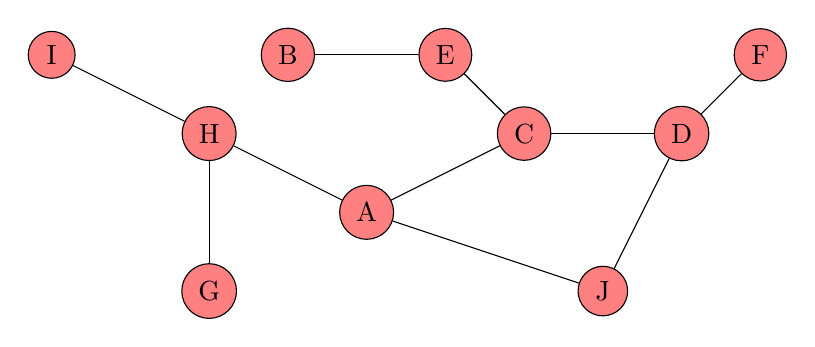
\begin{tikzpicture}
\node[draw,circle,fill=red!50] (A)at(0,0) {A};
\node[draw,circle,fill=red!50] (B)at(-1,2) {B};
\node[draw,circle,fill=red!50] (C)at(2,1) {C};
\node[draw,circle,fill=red!50] (D)at(4,1) {D};
\node[draw,circle,fill=red!50] (E)at(1,2) {E};
\node[draw,circle,fill=red!50] (F)at(5,2) {F};
\node[draw,circle,fill=red!50] (G)at(-2,-1) {G};
\node[draw,circle,fill=red!50] (H)at(-2,1) {H};
\node[draw,circle,fill=red!50] (I)at(-4,2) {I};
\node[draw,circle,fill=red!50] (J)at(3,-1) {J};
\draw[-,>=latex] (E) -- (B);
\draw[-,>=latex] (A) -- (C);
\draw[-,>=latex] (A) -- (H);
\draw[-,>=latex] (A) -- (J);
\draw[-,>=latex] (H) -- (I);
\draw[-,>=latex] (H) -- (G);
\draw[-,>=latex] (C) -- (E);
\draw[-,>=latex] (C) -- (D);
%\draw[-,>=latex] (C) -- (J);
\draw[-,>=latex] (D) -- (J);
\draw[-,>=latex] (D) -- (F);
\end{tikzpicture}
\end{center}
\pagebreak
BFS

\begin{center}
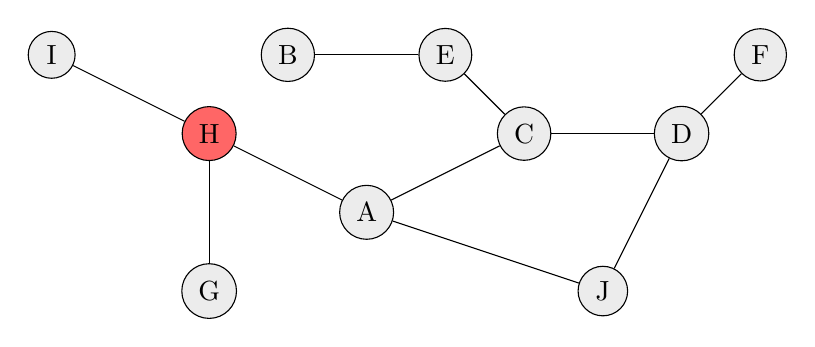
\begin{tikzpicture}
\node[draw,circle,fill=gray!15] (A)at(0,0) {A};
\node[draw,circle,fill=gray!15] (B)at(-1,2) {B};
\node[draw,circle,fill=gray!15] (C)at(2,1) {C};
\node[draw,circle,fill=gray!15] (D)at(4,1) {D};
\node[draw,circle,fill=gray!15] (E)at(1,2) {E};
\node[draw,circle,fill=gray!15] (F)at(5,2) {F};
\node[draw,circle,fill=gray!15] (G)at(-2,-1) {G};
\node[draw,circle,fill=red!60] (H)at(-2,1) {H};
\node[draw,circle,fill=gray!15] (I)at(-4,2) {I};
\node[draw,circle,fill=gray!15] (J)at(3,-1) {J};
\draw[-,>=latex] (E) -- (B);
\draw[-,>=latex] (A) -- (C);
\draw[-,>=latex] (A) -- (H);
\draw[-,>=latex] (A) -- (J);
\draw[-,>=latex] (H) -- (I);
\draw[-,>=latex] (H) -- (G);
\draw[-,>=latex] (C) -- (E);
\draw[-,>=latex] (C) -- (D);
%\draw[-,>=latex] (C) -- (J);
\draw[-,>=latex] (D) -- (J);
\draw[-,>=latex] (D) -- (F);
\end{tikzpicture}
\end{center}

\begin{center}
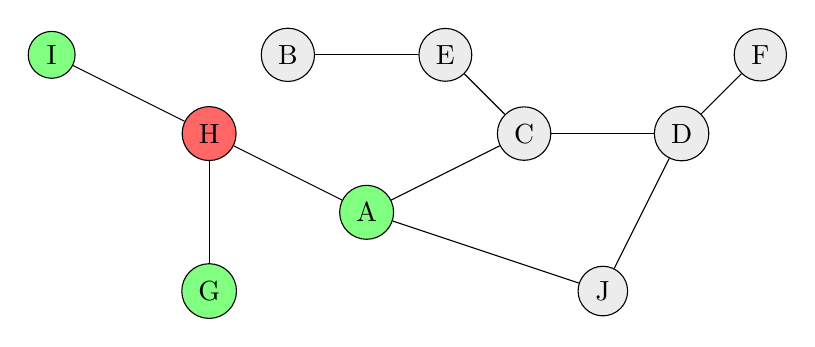
\begin{tikzpicture}
\node[draw,circle,fill=green!50] (A)at(0,0) {A};
\node[draw,circle,fill=gray!15] (B)at(-1,2) {B};
\node[draw,circle,fill=gray!15] (C)at(2,1) {C};
\node[draw,circle,fill=gray!15] (D)at(4,1) {D};
\node[draw,circle,fill=gray!15] (E)at(1,2) {E};
\node[draw,circle,fill=gray!15] (F)at(5,2) {F};
\node[draw,circle,fill=green!50] (G)at(-2,-1) {G};
\node[draw,circle,fill=red!60] (H)at(-2,1) {H};
\node[draw,circle,fill=green!50] (I)at(-4,2) {I};
\node[draw,circle,fill=gray!15] (J)at(3,-1) {J};
\draw[-,>=latex] (E) -- (B);
\draw[-,>=latex] (A) -- (C);
\draw[-,>=latex] (A) -- (H);
\draw[-,>=latex] (A) -- (J);
\draw[-,>=latex] (H) -- (I);
\draw[-,>=latex] (H) -- (G);
\draw[-,>=latex] (C) -- (E);
\draw[-,>=latex] (C) -- (D);
%\draw[-,>=latex] (C) -- (J);
\draw[-,>=latex] (D) -- (J);
\draw[-,>=latex] (D) -- (F);
\end{tikzpicture}
\end{center}

\begin{center}
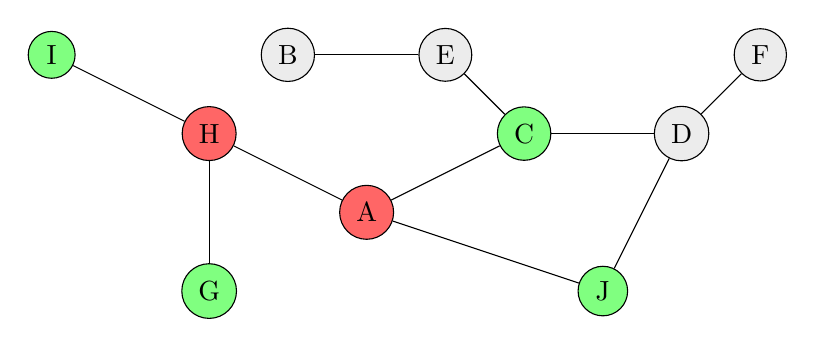
\begin{tikzpicture}
\node[draw,circle,fill=red!60] (A)at(0,0) {A};
\node[draw,circle,fill=gray!15] (B)at(-1,2) {B};
\node[draw,circle,fill=green!50] (C)at(2,1) {C};
\node[draw,circle,fill=gray!15] (D)at(4,1) {D};
\node[draw,circle,fill=gray!15] (E)at(1,2) {E};
\node[draw,circle,fill=gray!15] (F)at(5,2) {F};
\node[draw,circle,fill=green!50] (G)at(-2,-1) {G};
\node[draw,circle,fill=red!60] (H)at(-2,1) {H};
\node[draw,circle,fill=green!50] (I)at(-4,2) {I};
\node[draw,circle,fill=green!50] (J)at(3,-1) {J};
\draw[-,>=latex] (E) -- (B);
\draw[-,>=latex] (A) -- (C);
\draw[-,>=latex] (A) -- (H);
\draw[-,>=latex] (A) -- (J);
\draw[-,>=latex] (H) -- (I);
\draw[-,>=latex] (H) -- (G);
\draw[-,>=latex] (C) -- (E);
\draw[-,>=latex] (C) -- (D);
%\draw[-,>=latex] (C) -- (J);
\draw[-,>=latex] (D) -- (J);
\draw[-,>=latex] (D) -- (F);
\end{tikzpicture}
\end{center}

\begin{center}
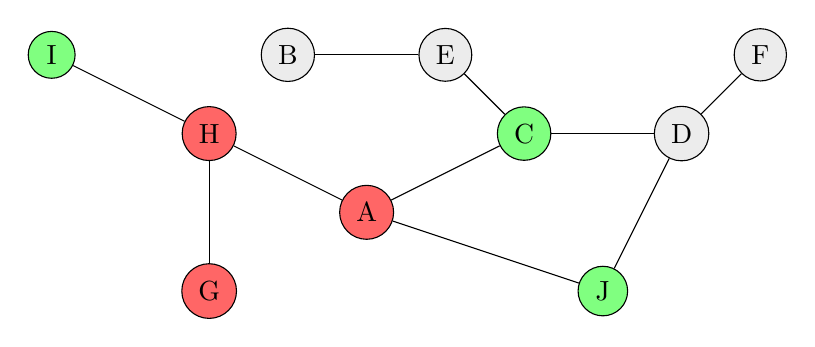
\begin{tikzpicture}
\node[draw,circle,fill=red!60] (A)at(0,0) {A};
\node[draw,circle,fill=gray!15] (B)at(-1,2) {B};
\node[draw,circle,fill=green!50] (C)at(2,1) {C};
\node[draw,circle,fill=gray!15] (D)at(4,1) {D};
\node[draw,circle,fill=gray!15] (E)at(1,2) {E};
\node[draw,circle,fill=gray!15] (F)at(5,2) {F};
\node[draw,circle,fill=red!60] (G)at(-2,-1) {G};
\node[draw,circle,fill=red!60] (H)at(-2,1) {H};
\node[draw,circle,fill=green!50] (I)at(-4,2) {I};
\node[draw,circle,fill=green!50] (J)at(3,-1) {J};
\draw[-,>=latex] (E) -- (B);
\draw[-,>=latex] (A) -- (C);
\draw[-,>=latex] (A) -- (H);
\draw[-,>=latex] (A) -- (J);
\draw[-,>=latex] (H) -- (I);
\draw[-,>=latex] (H) -- (G);
\draw[-,>=latex] (C) -- (E);
\draw[-,>=latex] (C) -- (D);
%\draw[-,>=latex] (C) -- (J);
\draw[-,>=latex] (D) -- (J);
\draw[-,>=latex] (D) -- (F);
\end{tikzpicture}
\end{center}

\begin{center}
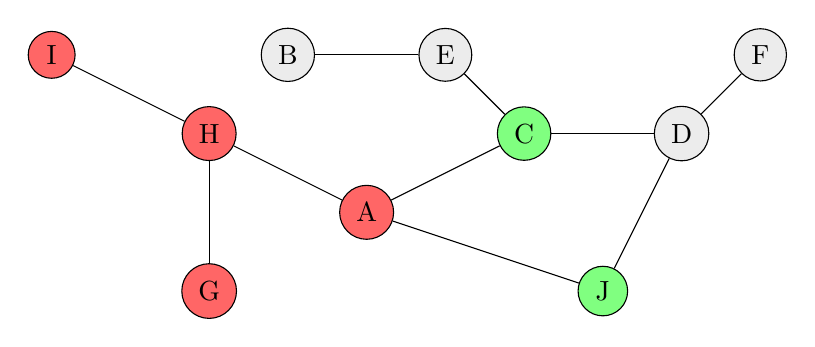
\begin{tikzpicture}
\node[draw,circle,fill=red!60] (A)at(0,0) {A};
\node[draw,circle,fill=gray!15] (B)at(-1,2) {B};
\node[draw,circle,fill=green!50] (C)at(2,1) {C};
\node[draw,circle,fill=gray!15] (D)at(4,1) {D};
\node[draw,circle,fill=gray!15] (E)at(1,2) {E};
\node[draw,circle,fill=gray!15] (F)at(5,2) {F};
\node[draw,circle,fill=red!60] (G)at(-2,-1) {G};
\node[draw,circle,fill=red!60] (H)at(-2,1) {H};
\node[draw,circle,fill=red!60] (I)at(-4,2) {I};
\node[draw,circle,fill=green!50] (J)at(3,-1) {J};
\draw[-,>=latex] (E) -- (B);
\draw[-,>=latex] (A) -- (C);
\draw[-,>=latex] (A) -- (H);
\draw[-,>=latex] (A) -- (J);
\draw[-,>=latex] (H) -- (I);
\draw[-,>=latex] (H) -- (G);
\draw[-,>=latex] (C) -- (E);
\draw[-,>=latex] (C) -- (D);
%\draw[-,>=latex] (C) -- (J);
\draw[-,>=latex] (D) -- (J);
\draw[-,>=latex] (D) -- (F);
\end{tikzpicture}
\end{center}

\begin{center}
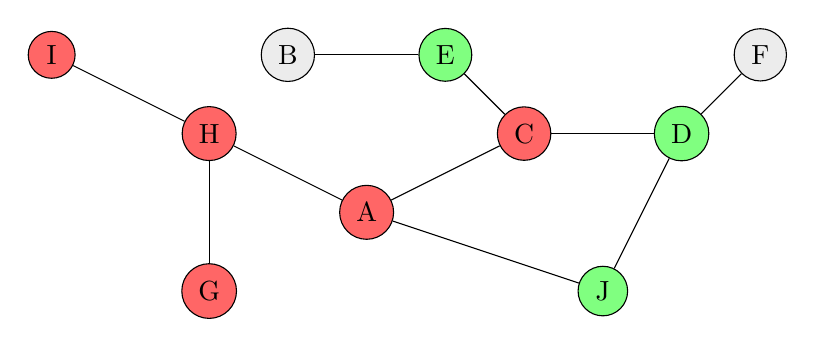
\begin{tikzpicture}
\node[draw,circle,fill=red!60] (A)at(0,0) {A};
\node[draw,circle,fill=gray!15] (B)at(-1,2) {B};
\node[draw,circle,fill=red!60] (C)at(2,1) {C};
\node[draw,circle,fill=green!50] (D)at(4,1) {D};
\node[draw,circle,fill=green!50] (E)at(1,2) {E};
\node[draw,circle,fill=gray!15] (F)at(5,2) {F};
\node[draw,circle,fill=red!60] (G)at(-2,-1) {G};
\node[draw,circle,fill=red!60] (H)at(-2,1) {H};
\node[draw,circle,fill=red!60] (I)at(-4,2) {I};
\node[draw,circle,fill=green!50] (J)at(3,-1) {J};
\draw[-,>=latex] (E) -- (B);
\draw[-,>=latex] (A) -- (C);
\draw[-,>=latex] (A) -- (H);
\draw[-,>=latex] (A) -- (J);
\draw[-,>=latex] (H) -- (I);
\draw[-,>=latex] (H) -- (G);
\draw[-,>=latex] (C) -- (E);
\draw[-,>=latex] (C) -- (D);
%\draw[-,>=latex] (C) -- (J);
\draw[-,>=latex] (D) -- (J);
\draw[-,>=latex] (D) -- (F);
\end{tikzpicture}
\end{center}

\begin{center}
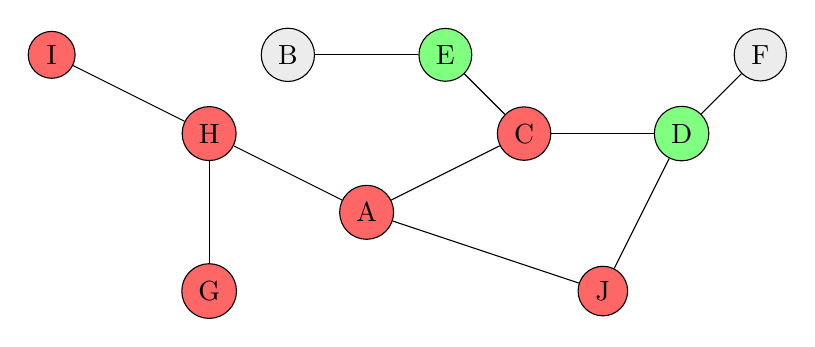
\begin{tikzpicture}
\node[draw,circle,fill=red!60] (A)at(0,0) {A};
\node[draw,circle,fill=gray!15] (B)at(-1,2) {B};
\node[draw,circle,fill=red!60] (C)at(2,1) {C};
\node[draw,circle,fill=green!50] (D)at(4,1) {D};
\node[draw,circle,fill=green!50] (E)at(1,2) {E};
\node[draw,circle,fill=gray!15] (F)at(5,2) {F};
\node[draw,circle,fill=red!60] (G)at(-2,-1) {G};
\node[draw,circle,fill=red!60] (H)at(-2,1) {H};
\node[draw,circle,fill=red!60] (I)at(-4,2) {I};
\node[draw,circle,fill=red!60] (J)at(3,-1) {J};
\draw[-,>=latex] (E) -- (B);
\draw[-,>=latex] (A) -- (C);
\draw[-,>=latex] (A) -- (H);
\draw[-,>=latex] (A) -- (J);
\draw[-,>=latex] (H) -- (I);
\draw[-,>=latex] (H) -- (G);
\draw[-,>=latex] (C) -- (E);
\draw[-,>=latex] (C) -- (D);
%\draw[-,>=latex] (C) -- (J);
\draw[-,>=latex] (D) -- (J);
\draw[-,>=latex] (D) -- (F);
\end{tikzpicture}
\end{center}

\begin{center}
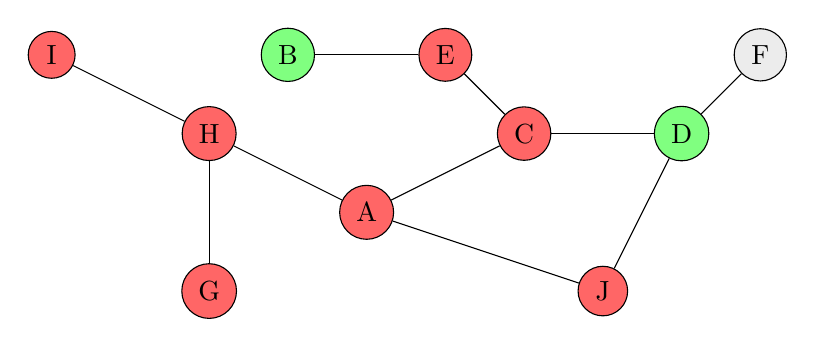
\begin{tikzpicture}
\node[draw,circle,fill=red!60] (A)at(0,0) {A};
\node[draw,circle,fill=green!50] (B)at(-1,2) {B};
\node[draw,circle,fill=red!60] (C)at(2,1) {C};
\node[draw,circle,fill=green!50] (D)at(4,1) {D};
\node[draw,circle,fill=red!60] (E)at(1,2) {E};
\node[draw,circle,fill=gray!15] (F)at(5,2) {F};
\node[draw,circle,fill=red!60] (G)at(-2,-1) {G};
\node[draw,circle,fill=red!60] (H)at(-2,1) {H};
\node[draw,circle,fill=red!60] (I)at(-4,2) {I};
\node[draw,circle,fill=red!60] (J)at(3,-1) {J};
\draw[-,>=latex] (E) -- (B);
\draw[-,>=latex] (A) -- (C);
\draw[-,>=latex] (A) -- (H);
\draw[-,>=latex] (A) -- (J);
\draw[-,>=latex] (H) -- (I);
\draw[-,>=latex] (H) -- (G);
\draw[-,>=latex] (C) -- (E);
\draw[-,>=latex] (C) -- (D);
%\draw[-,>=latex] (C) -- (J);
\draw[-,>=latex] (D) -- (J);
\draw[-,>=latex] (D) -- (F);
\end{tikzpicture}
\end{center}

\begin{center}
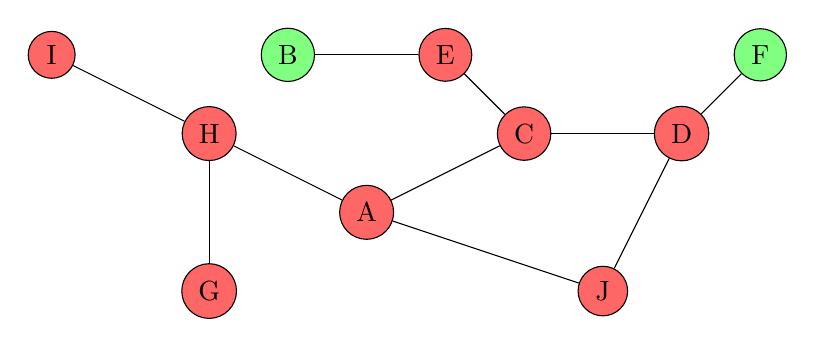
\begin{tikzpicture}
\node[draw,circle,fill=red!60] (A)at(0,0) {A};
\node[draw,circle,fill=green!50] (B)at(-1,2) {B};
\node[draw,circle,fill=red!60] (C)at(2,1) {C};
\node[draw,circle,fill=red!60] (D)at(4,1) {D};
\node[draw,circle,fill=red!60] (E)at(1,2) {E};
\node[draw,circle,fill=green!50] (F)at(5,2) {F};
\node[draw,circle,fill=red!60] (G)at(-2,-1) {G};
\node[draw,circle,fill=red!60] (H)at(-2,1) {H};
\node[draw,circle,fill=red!60] (I)at(-4,2) {I};
\node[draw,circle,fill=red!60] (J)at(3,-1) {J};
\draw[-,>=latex] (E) -- (B);
\draw[-,>=latex] (A) -- (C);
\draw[-,>=latex] (A) -- (H);
\draw[-,>=latex] (A) -- (J);
\draw[-,>=latex] (H) -- (I);
\draw[-,>=latex] (H) -- (G);
\draw[-,>=latex] (C) -- (E);
\draw[-,>=latex] (C) -- (D);
%\draw[-,>=latex] (C) -- (J);
\draw[-,>=latex] (D) -- (J);
\draw[-,>=latex] (D) -- (F);
\end{tikzpicture}
\end{center}

\begin{center}
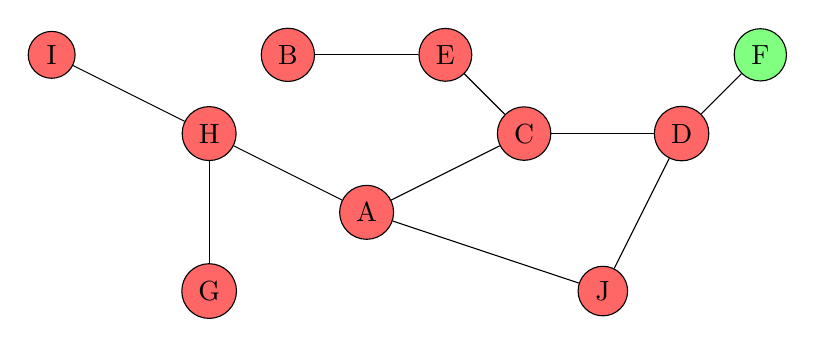
\begin{tikzpicture}
\node[draw,circle,fill=red!60] (A)at(0,0) {A};
\node[draw,circle,fill=red!60] (B)at(-1,2) {B};
\node[draw,circle,fill=red!60] (C)at(2,1) {C};
\node[draw,circle,fill=red!60] (D)at(4,1) {D};
\node[draw,circle,fill=red!60] (E)at(1,2) {E};
\node[draw,circle,fill=green!50] (F)at(5,2) {F};
\node[draw,circle,fill=red!60] (G)at(-2,-1) {G};
\node[draw,circle,fill=red!60] (H)at(-2,1) {H};
\node[draw,circle,fill=red!60] (I)at(-4,2) {I};
\node[draw,circle,fill=red!60] (J)at(3,-1) {J};
\draw[-,>=latex] (E) -- (B);
\draw[-,>=latex] (A) -- (C);
\draw[-,>=latex] (A) -- (H);
\draw[-,>=latex] (A) -- (J);
\draw[-,>=latex] (H) -- (I);
\draw[-,>=latex] (H) -- (G);
\draw[-,>=latex] (C) -- (E);
\draw[-,>=latex] (C) -- (D);
%\draw[-,>=latex] (C) -- (J);
\draw[-,>=latex] (D) -- (J);
\draw[-,>=latex] (D) -- (F);
\end{tikzpicture}
\end{center}

\begin{center}
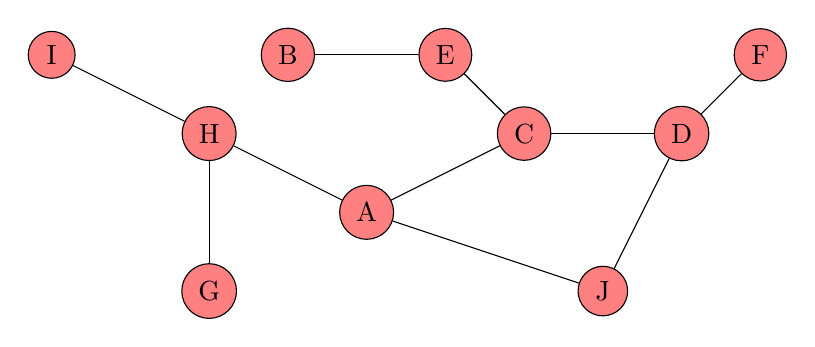
\begin{tikzpicture}
\node[draw,circle,fill=red!50] (A)at(0,0) {A};
\node[draw,circle,fill=red!50] (B)at(-1,2) {B};
\node[draw,circle,fill=red!50] (C)at(2,1) {C};
\node[draw,circle,fill=red!50] (D)at(4,1) {D};
\node[draw,circle,fill=red!50] (E)at(1,2) {E};
\node[draw,circle,fill=red!50] (F)at(5,2) {F};
\node[draw,circle,fill=red!50] (G)at(-2,-1) {G};
\node[draw,circle,fill=red!50] (H)at(-2,1) {H};
\node[draw,circle,fill=red!50] (I)at(-4,2) {I};
\node[draw,circle,fill=red!50] (J)at(3,-1) {J};
\draw[-,>=latex] (E) -- (B);
\draw[-,>=latex] (A) -- (C);
\draw[-,>=latex] (A) -- (H);
\draw[-,>=latex] (A) -- (J);
\draw[-,>=latex] (H) -- (I);
\draw[-,>=latex] (H) -- (G);
\draw[-,>=latex] (C) -- (E);
\draw[-,>=latex] (C) -- (D);
%\draw[-,>=latex] (C) -- (J);
\draw[-,>=latex] (D) -- (J);
\draw[-,>=latex] (D) -- (F);
\end{tikzpicture}
\end{center}
\end{Form}
\end{document}